\chapter{Related Work}

%\subsubsection{Psychoacoustic Features and Gray Codes}

% This chapter covers relevant (and typically, recent) research
% which you build upon (or improve upon). There are two complementary
% goals for this chapter:
% \begin{enumerate}
%   \item to show that you know and understand the state of the art; and
%   \item to put your work in context
% \end{enumerate}

% Ideally you can tackle both together by providing a critique of
% related work, and describing what is insufficient (and how you do
% better!)

% The related work chapter should usually come either near the front or
% near the back of the dissertation. The advantage of the former is that
% you get to build the argument for why your work is important before
% presenting your solution(s) in later chapters; the advantage of the
% latter is that don't have to forward reference to your solution too
% much. The correct choice will depend on what you're writing up, and
% your own personal preference.


\section{RNNs}

\begin{enumerate}
    \item Bidirectional RNNs
        \begin{figure}[htpb]
            \centering
            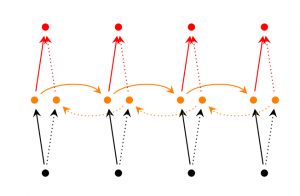
\includegraphics[width=0.8\linewidth]{Figures/bi-rnn.png}
            \caption{\todo{Redraw}}
        \end{figure}
        Cannot be sampled, but if the source sequence is given can run FW and BW LSTMs
        to obtain $\s^{FW}$ and $\s^{BW}$ then $\o_t = \softmax(V [\s^{FW}_; \s^{BW}_t])$
    \item Deep RNNs
        \begin{figure}[htpb]
            \centering
            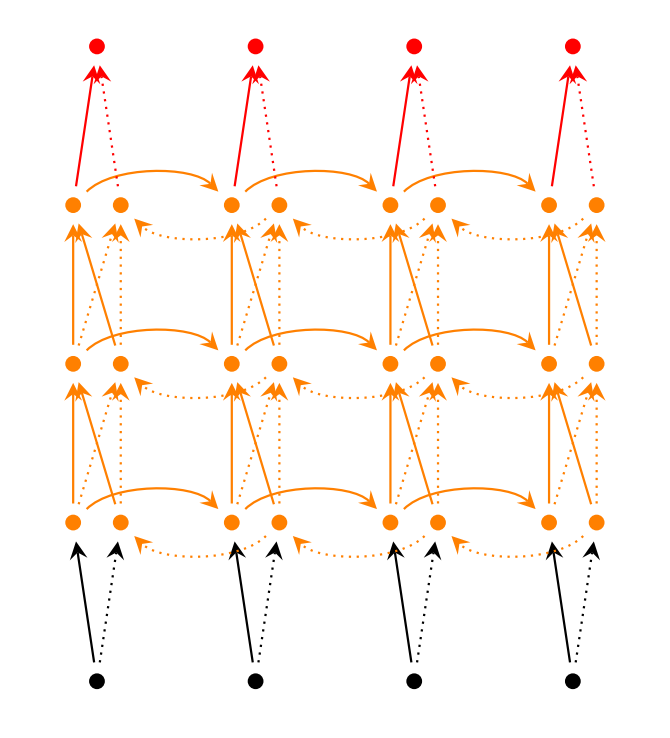
\includegraphics[width=0.8\linewidth]{Figures/deep-rnn.png}
            \caption{\todo{Redraw}}
        \end{figure}
        Outputs of one LSTM are used as inputs to the next; more layers $\implies$
        greater representational power, hierarchical representation learning?
    \item LSTMs
        \begin{enumerate}
            \item Memory is called \emph{cells}
        \end{enumerate}

    \item LSTM Variants: GRUs have fewer parameters (U and W are smaller) and
        thus may train a bit faster or need less data to generalize
\end{enumerate}

\subsection{RNN-RBM}
An alternative design is to have the RNN output the entire chord at teach time.
This is appealing because the steps between successive RNN applications
correspond to units of time. Additionaly, the emission distribution's parameterization
can be used to restrict the number of simultaneous parts.

In a RNN-RBM, the hidden state is used to compute the parameters for a restricted Boltzmann
machine at each timestep. The RBM parameterizess a multivariate categorical distribution,
which can be either over the four parts or the entire piano roll.


